\documentclass[border=6pt]{standalone}
\usepackage[utf8]{inputenc}\usepackage[T1]{fontenc}\usepackage{lmodern}\usepackage[english]{babel}
\usepackage{amsmath,amssymb}\usepackage{tikz}\usetikzlibrary{arrows.meta,positioning,calc,decorations.pathreplacing}
\begin{document}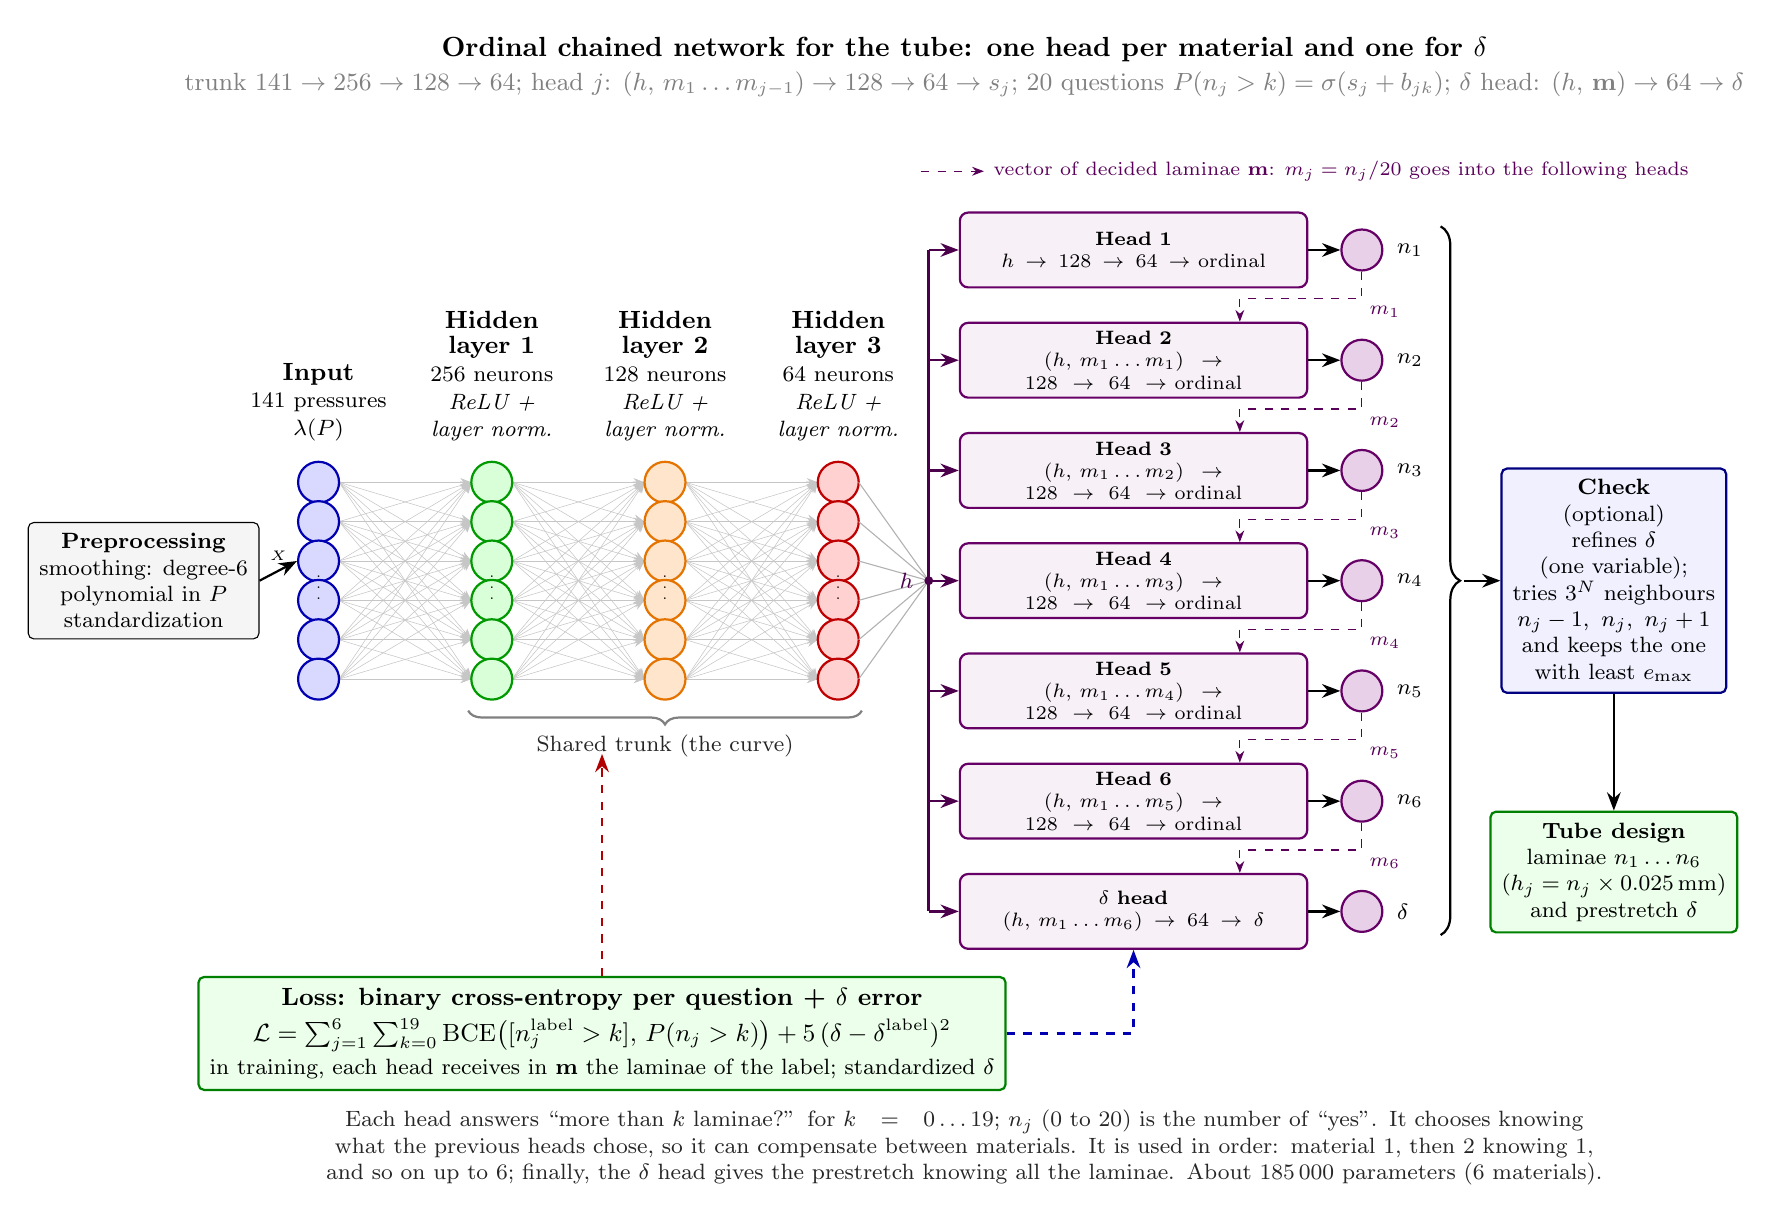
\begin{tikzpicture}[font=\small, n/.style={circle,draw,thick,minimum size=5.2mm,inner sep=0pt},
 box/.style={draw,rounded corners=2pt,fill=gray!8,align=center,inner sep=4pt,font=\footnotesize},
 hd/.style={draw=violet!80!black,thick,rounded corners=3pt,fill=violet!6,align=center,inner sep=3pt,font=\scriptsize,text width=4.2cm,minimum height=0.95cm}]
\node[font=\bfseries\normalsize] at (8.2,6.75) {Ordinal chained network for the tube: one head per material and one for $\delta$};
\node[gray] at (8.2,6.3) {trunk $141\to256\to128\to64$; head $j$: $(h,\,m_1\ldots m_{j-1})\to128\to64\to s_j$; 20 questions $P(n_j>k)=\sigma(s_j+b_{jk})$; $\delta$ head: $(h,\,\mathbf{m})\to64\to\delta$};
\draw[-{Stealth[length=1.4mm]},gray!45,very thin] (0.26,1.25)--(1.94,1.25);
\draw[-{Stealth[length=1.4mm]},gray!45,very thin] (0.26,1.25)--(1.94,0.75);
\draw[-{Stealth[length=1.4mm]},gray!45,very thin] (0.26,1.25)--(1.94,0.25);
\draw[-{Stealth[length=1.4mm]},gray!45,very thin] (0.26,1.25)--(1.94,-0.25);
\draw[-{Stealth[length=1.4mm]},gray!45,very thin] (0.26,1.25)--(1.94,-0.75);
\draw[-{Stealth[length=1.4mm]},gray!45,very thin] (0.26,1.25)--(1.94,-1.25);
\draw[-{Stealth[length=1.4mm]},gray!45,very thin] (0.26,0.75)--(1.94,1.25);
\draw[-{Stealth[length=1.4mm]},gray!45,very thin] (0.26,0.75)--(1.94,0.75);
\draw[-{Stealth[length=1.4mm]},gray!45,very thin] (0.26,0.75)--(1.94,0.25);
\draw[-{Stealth[length=1.4mm]},gray!45,very thin] (0.26,0.75)--(1.94,-0.25);
\draw[-{Stealth[length=1.4mm]},gray!45,very thin] (0.26,0.75)--(1.94,-0.75);
\draw[-{Stealth[length=1.4mm]},gray!45,very thin] (0.26,0.75)--(1.94,-1.25);
\draw[-{Stealth[length=1.4mm]},gray!45,very thin] (0.26,0.25)--(1.94,1.25);
\draw[-{Stealth[length=1.4mm]},gray!45,very thin] (0.26,0.25)--(1.94,0.75);
\draw[-{Stealth[length=1.4mm]},gray!45,very thin] (0.26,0.25)--(1.94,0.25);
\draw[-{Stealth[length=1.4mm]},gray!45,very thin] (0.26,0.25)--(1.94,-0.25);
\draw[-{Stealth[length=1.4mm]},gray!45,very thin] (0.26,0.25)--(1.94,-0.75);
\draw[-{Stealth[length=1.4mm]},gray!45,very thin] (0.26,0.25)--(1.94,-1.25);
\draw[-{Stealth[length=1.4mm]},gray!45,very thin] (0.26,-0.25)--(1.94,1.25);
\draw[-{Stealth[length=1.4mm]},gray!45,very thin] (0.26,-0.25)--(1.94,0.75);
\draw[-{Stealth[length=1.4mm]},gray!45,very thin] (0.26,-0.25)--(1.94,0.25);
\draw[-{Stealth[length=1.4mm]},gray!45,very thin] (0.26,-0.25)--(1.94,-0.25);
\draw[-{Stealth[length=1.4mm]},gray!45,very thin] (0.26,-0.25)--(1.94,-0.75);
\draw[-{Stealth[length=1.4mm]},gray!45,very thin] (0.26,-0.25)--(1.94,-1.25);
\draw[-{Stealth[length=1.4mm]},gray!45,very thin] (0.26,-0.75)--(1.94,1.25);
\draw[-{Stealth[length=1.4mm]},gray!45,very thin] (0.26,-0.75)--(1.94,0.75);
\draw[-{Stealth[length=1.4mm]},gray!45,very thin] (0.26,-0.75)--(1.94,0.25);
\draw[-{Stealth[length=1.4mm]},gray!45,very thin] (0.26,-0.75)--(1.94,-0.25);
\draw[-{Stealth[length=1.4mm]},gray!45,very thin] (0.26,-0.75)--(1.94,-0.75);
\draw[-{Stealth[length=1.4mm]},gray!45,very thin] (0.26,-0.75)--(1.94,-1.25);
\draw[-{Stealth[length=1.4mm]},gray!45,very thin] (0.26,-1.25)--(1.94,1.25);
\draw[-{Stealth[length=1.4mm]},gray!45,very thin] (0.26,-1.25)--(1.94,0.75);
\draw[-{Stealth[length=1.4mm]},gray!45,very thin] (0.26,-1.25)--(1.94,0.25);
\draw[-{Stealth[length=1.4mm]},gray!45,very thin] (0.26,-1.25)--(1.94,-0.25);
\draw[-{Stealth[length=1.4mm]},gray!45,very thin] (0.26,-1.25)--(1.94,-0.75);
\draw[-{Stealth[length=1.4mm]},gray!45,very thin] (0.26,-1.25)--(1.94,-1.25);
\draw[-{Stealth[length=1.4mm]},gray!45,very thin] (2.46,1.25)--(4.14,1.25);
\draw[-{Stealth[length=1.4mm]},gray!45,very thin] (2.46,1.25)--(4.14,0.75);
\draw[-{Stealth[length=1.4mm]},gray!45,very thin] (2.46,1.25)--(4.14,0.25);
\draw[-{Stealth[length=1.4mm]},gray!45,very thin] (2.46,1.25)--(4.14,-0.25);
\draw[-{Stealth[length=1.4mm]},gray!45,very thin] (2.46,1.25)--(4.14,-0.75);
\draw[-{Stealth[length=1.4mm]},gray!45,very thin] (2.46,1.25)--(4.14,-1.25);
\draw[-{Stealth[length=1.4mm]},gray!45,very thin] (2.46,0.75)--(4.14,1.25);
\draw[-{Stealth[length=1.4mm]},gray!45,very thin] (2.46,0.75)--(4.14,0.75);
\draw[-{Stealth[length=1.4mm]},gray!45,very thin] (2.46,0.75)--(4.14,0.25);
\draw[-{Stealth[length=1.4mm]},gray!45,very thin] (2.46,0.75)--(4.14,-0.25);
\draw[-{Stealth[length=1.4mm]},gray!45,very thin] (2.46,0.75)--(4.14,-0.75);
\draw[-{Stealth[length=1.4mm]},gray!45,very thin] (2.46,0.75)--(4.14,-1.25);
\draw[-{Stealth[length=1.4mm]},gray!45,very thin] (2.46,0.25)--(4.14,1.25);
\draw[-{Stealth[length=1.4mm]},gray!45,very thin] (2.46,0.25)--(4.14,0.75);
\draw[-{Stealth[length=1.4mm]},gray!45,very thin] (2.46,0.25)--(4.14,0.25);
\draw[-{Stealth[length=1.4mm]},gray!45,very thin] (2.46,0.25)--(4.14,-0.25);
\draw[-{Stealth[length=1.4mm]},gray!45,very thin] (2.46,0.25)--(4.14,-0.75);
\draw[-{Stealth[length=1.4mm]},gray!45,very thin] (2.46,0.25)--(4.14,-1.25);
\draw[-{Stealth[length=1.4mm]},gray!45,very thin] (2.46,-0.25)--(4.14,1.25);
\draw[-{Stealth[length=1.4mm]},gray!45,very thin] (2.46,-0.25)--(4.14,0.75);
\draw[-{Stealth[length=1.4mm]},gray!45,very thin] (2.46,-0.25)--(4.14,0.25);
\draw[-{Stealth[length=1.4mm]},gray!45,very thin] (2.46,-0.25)--(4.14,-0.25);
\draw[-{Stealth[length=1.4mm]},gray!45,very thin] (2.46,-0.25)--(4.14,-0.75);
\draw[-{Stealth[length=1.4mm]},gray!45,very thin] (2.46,-0.25)--(4.14,-1.25);
\draw[-{Stealth[length=1.4mm]},gray!45,very thin] (2.46,-0.75)--(4.14,1.25);
\draw[-{Stealth[length=1.4mm]},gray!45,very thin] (2.46,-0.75)--(4.14,0.75);
\draw[-{Stealth[length=1.4mm]},gray!45,very thin] (2.46,-0.75)--(4.14,0.25);
\draw[-{Stealth[length=1.4mm]},gray!45,very thin] (2.46,-0.75)--(4.14,-0.25);
\draw[-{Stealth[length=1.4mm]},gray!45,very thin] (2.46,-0.75)--(4.14,-0.75);
\draw[-{Stealth[length=1.4mm]},gray!45,very thin] (2.46,-0.75)--(4.14,-1.25);
\draw[-{Stealth[length=1.4mm]},gray!45,very thin] (2.46,-1.25)--(4.14,1.25);
\draw[-{Stealth[length=1.4mm]},gray!45,very thin] (2.46,-1.25)--(4.14,0.75);
\draw[-{Stealth[length=1.4mm]},gray!45,very thin] (2.46,-1.25)--(4.14,0.25);
\draw[-{Stealth[length=1.4mm]},gray!45,very thin] (2.46,-1.25)--(4.14,-0.25);
\draw[-{Stealth[length=1.4mm]},gray!45,very thin] (2.46,-1.25)--(4.14,-0.75);
\draw[-{Stealth[length=1.4mm]},gray!45,very thin] (2.46,-1.25)--(4.14,-1.25);
\draw[-{Stealth[length=1.4mm]},gray!45,very thin] (4.66,1.25)--(6.34,1.25);
\draw[-{Stealth[length=1.4mm]},gray!45,very thin] (4.66,1.25)--(6.34,0.75);
\draw[-{Stealth[length=1.4mm]},gray!45,very thin] (4.66,1.25)--(6.34,0.25);
\draw[-{Stealth[length=1.4mm]},gray!45,very thin] (4.66,1.25)--(6.34,-0.25);
\draw[-{Stealth[length=1.4mm]},gray!45,very thin] (4.66,1.25)--(6.34,-0.75);
\draw[-{Stealth[length=1.4mm]},gray!45,very thin] (4.66,1.25)--(6.34,-1.25);
\draw[-{Stealth[length=1.4mm]},gray!45,very thin] (4.66,0.75)--(6.34,1.25);
\draw[-{Stealth[length=1.4mm]},gray!45,very thin] (4.66,0.75)--(6.34,0.75);
\draw[-{Stealth[length=1.4mm]},gray!45,very thin] (4.66,0.75)--(6.34,0.25);
\draw[-{Stealth[length=1.4mm]},gray!45,very thin] (4.66,0.75)--(6.34,-0.25);
\draw[-{Stealth[length=1.4mm]},gray!45,very thin] (4.66,0.75)--(6.34,-0.75);
\draw[-{Stealth[length=1.4mm]},gray!45,very thin] (4.66,0.75)--(6.34,-1.25);
\draw[-{Stealth[length=1.4mm]},gray!45,very thin] (4.66,0.25)--(6.34,1.25);
\draw[-{Stealth[length=1.4mm]},gray!45,very thin] (4.66,0.25)--(6.34,0.75);
\draw[-{Stealth[length=1.4mm]},gray!45,very thin] (4.66,0.25)--(6.34,0.25);
\draw[-{Stealth[length=1.4mm]},gray!45,very thin] (4.66,0.25)--(6.34,-0.25);
\draw[-{Stealth[length=1.4mm]},gray!45,very thin] (4.66,0.25)--(6.34,-0.75);
\draw[-{Stealth[length=1.4mm]},gray!45,very thin] (4.66,0.25)--(6.34,-1.25);
\draw[-{Stealth[length=1.4mm]},gray!45,very thin] (4.66,-0.25)--(6.34,1.25);
\draw[-{Stealth[length=1.4mm]},gray!45,very thin] (4.66,-0.25)--(6.34,0.75);
\draw[-{Stealth[length=1.4mm]},gray!45,very thin] (4.66,-0.25)--(6.34,0.25);
\draw[-{Stealth[length=1.4mm]},gray!45,very thin] (4.66,-0.25)--(6.34,-0.25);
\draw[-{Stealth[length=1.4mm]},gray!45,very thin] (4.66,-0.25)--(6.34,-0.75);
\draw[-{Stealth[length=1.4mm]},gray!45,very thin] (4.66,-0.25)--(6.34,-1.25);
\draw[-{Stealth[length=1.4mm]},gray!45,very thin] (4.66,-0.75)--(6.34,1.25);
\draw[-{Stealth[length=1.4mm]},gray!45,very thin] (4.66,-0.75)--(6.34,0.75);
\draw[-{Stealth[length=1.4mm]},gray!45,very thin] (4.66,-0.75)--(6.34,0.25);
\draw[-{Stealth[length=1.4mm]},gray!45,very thin] (4.66,-0.75)--(6.34,-0.25);
\draw[-{Stealth[length=1.4mm]},gray!45,very thin] (4.66,-0.75)--(6.34,-0.75);
\draw[-{Stealth[length=1.4mm]},gray!45,very thin] (4.66,-0.75)--(6.34,-1.25);
\draw[-{Stealth[length=1.4mm]},gray!45,very thin] (4.66,-1.25)--(6.34,1.25);
\draw[-{Stealth[length=1.4mm]},gray!45,very thin] (4.66,-1.25)--(6.34,0.75);
\draw[-{Stealth[length=1.4mm]},gray!45,very thin] (4.66,-1.25)--(6.34,0.25);
\draw[-{Stealth[length=1.4mm]},gray!45,very thin] (4.66,-1.25)--(6.34,-0.25);
\draw[-{Stealth[length=1.4mm]},gray!45,very thin] (4.66,-1.25)--(6.34,-0.75);
\draw[-{Stealth[length=1.4mm]},gray!45,very thin] (4.66,-1.25)--(6.34,-1.25);
\node[n,draw=blue!70!black,fill=blue!15] (n00) at (0.00,1.25) {};
\node[n,draw=blue!70!black,fill=blue!15] (n01) at (0.00,0.75) {};
\node[n,draw=blue!70!black,fill=blue!15] (n02) at (0.00,0.25) {};
\node[n,draw=blue!70!black,fill=blue!15] (n03) at (0.00,-0.25) {};
\node[n,draw=blue!70!black,fill=blue!15] (n04) at (0.00,-0.75) {};
\node[n,draw=blue!70!black,fill=blue!15] (n05) at (0.00,-1.25) {};
\node[font=\tiny] at (0.00,0.02) {$\vdots$};
\node[align=center,anchor=south] at (0.00,1.65) {\textbf{Input}\\[-1pt]\footnotesize 141 pressures\\[-1pt]\footnotesize\itshape $\lambda(P)$};
\node[n,draw=green!60!black,fill=green!15] (n10) at (2.20,1.25) {};
\node[n,draw=green!60!black,fill=green!15] (n11) at (2.20,0.75) {};
\node[n,draw=green!60!black,fill=green!15] (n12) at (2.20,0.25) {};
\node[n,draw=green!60!black,fill=green!15] (n13) at (2.20,-0.25) {};
\node[n,draw=green!60!black,fill=green!15] (n14) at (2.20,-0.75) {};
\node[n,draw=green!60!black,fill=green!15] (n15) at (2.20,-1.25) {};
\node[font=\tiny] at (2.20,0.02) {$\vdots$};
\node[align=center,anchor=south] at (2.20,1.65) {\textbf{\shortstack{Hidden\\layer 1}}\\[-1pt]\footnotesize 256 neurons\\[-1pt]\footnotesize\itshape ReLU +\\[-1pt]\footnotesize\itshape layer norm.};
\node[n,draw=orange!90!black,fill=orange!20] (n20) at (4.40,1.25) {};
\node[n,draw=orange!90!black,fill=orange!20] (n21) at (4.40,0.75) {};
\node[n,draw=orange!90!black,fill=orange!20] (n22) at (4.40,0.25) {};
\node[n,draw=orange!90!black,fill=orange!20] (n23) at (4.40,-0.25) {};
\node[n,draw=orange!90!black,fill=orange!20] (n24) at (4.40,-0.75) {};
\node[n,draw=orange!90!black,fill=orange!20] (n25) at (4.40,-1.25) {};
\node[font=\tiny] at (4.40,0.02) {$\vdots$};
\node[align=center,anchor=south] at (4.40,1.65) {\textbf{\shortstack{Hidden\\layer 2}}\\[-1pt]\footnotesize 128 neurons\\[-1pt]\footnotesize\itshape ReLU +\\[-1pt]\footnotesize\itshape layer norm.};
\node[n,draw=red!75!black,fill=red!18] (n30) at (6.60,1.25) {};
\node[n,draw=red!75!black,fill=red!18] (n31) at (6.60,0.75) {};
\node[n,draw=red!75!black,fill=red!18] (n32) at (6.60,0.25) {};
\node[n,draw=red!75!black,fill=red!18] (n33) at (6.60,-0.25) {};
\node[n,draw=red!75!black,fill=red!18] (n34) at (6.60,-0.75) {};
\node[n,draw=red!75!black,fill=red!18] (n35) at (6.60,-1.25) {};
\node[font=\tiny] at (6.60,0.02) {$\vdots$};
\node[align=center,anchor=south] at (6.60,1.65) {\textbf{\shortstack{Hidden\\layer 3}}\\[-1pt]\footnotesize 64 neurons\\[-1pt]\footnotesize\itshape ReLU +\\[-1pt]\footnotesize\itshape layer norm.};
\draw[decorate,decoration={brace,mirror,amplitude=5pt},thick,gray] (1.9,-1.65)--(6.9,-1.65) node[midway,below=5pt,font=\footnotesize,gray!30!black] {Shared trunk (the curve)};
\draw[gray!60,thin] (6.86,1.25)--(7.75,0);
\draw[gray!60,thin] (6.86,0.75)--(7.75,0);
\draw[gray!60,thin] (6.86,0.25)--(7.75,0);
\draw[gray!60,thin] (6.86,-0.25)--(7.75,0);
\draw[gray!60,thin] (6.86,-0.75)--(7.75,0);
\draw[gray!60,thin] (6.86,-1.25)--(7.75,0);
\draw[very thick,violet!60!black] (7.75,4.20)--(7.75,-4.20);
\fill[violet!60!black] (7.75,0) circle (1.6pt) node[left=2pt,font=\footnotesize] {$h$};
\node[hd] (h1) at (10.35,4.20) {\textbf{Head 1}\\ $h\to128\to64\to$ ordinal};
\draw[-{Stealth},thick,violet!60!black] (7.75,4.20)--(h1.west);
\node[n,draw=violet!80!black,fill=violet!18] (o1) at (13.25,4.20) {};
\node[right=0.5mm of o1,font=\footnotesize] {$n_{1}$};
\draw[-{Stealth},thick] (h1.east)--(o1.west);
\node[hd] (h2) at (10.35,2.80) {\textbf{Head 2}\\ $(h,\,m_1\ldots m_{1})\to128\to64\to$ ordinal};
\draw[-{Stealth},thick,violet!60!black] (7.75,2.80)--(h2.west);
\node[n,draw=violet!80!black,fill=violet!18] (o2) at (13.25,2.80) {};
\node[right=0.5mm of o2,font=\footnotesize] {$n_{2}$};
\draw[-{Stealth},thick] (h2.east)--(o2.west);
\node[hd] (h3) at (10.35,1.40) {\textbf{Head 3}\\ $(h,\,m_1\ldots m_{2})\to128\to64\to$ ordinal};
\draw[-{Stealth},thick,violet!60!black] (7.75,1.40)--(h3.west);
\node[n,draw=violet!80!black,fill=violet!18] (o3) at (13.25,1.40) {};
\node[right=0.5mm of o3,font=\footnotesize] {$n_{3}$};
\draw[-{Stealth},thick] (h3.east)--(o3.west);
\node[hd] (h4) at (10.35,0.00) {\textbf{Head 4}\\ $(h,\,m_1\ldots m_{3})\to128\to64\to$ ordinal};
\draw[-{Stealth},thick,violet!60!black] (7.75,0.00)--(h4.west);
\node[n,draw=violet!80!black,fill=violet!18] (o4) at (13.25,0.00) {};
\node[right=0.5mm of o4,font=\footnotesize] {$n_{4}$};
\draw[-{Stealth},thick] (h4.east)--(o4.west);
\node[hd] (h5) at (10.35,-1.40) {\textbf{Head 5}\\ $(h,\,m_1\ldots m_{4})\to128\to64\to$ ordinal};
\draw[-{Stealth},thick,violet!60!black] (7.75,-1.40)--(h5.west);
\node[n,draw=violet!80!black,fill=violet!18] (o5) at (13.25,-1.40) {};
\node[right=0.5mm of o5,font=\footnotesize] {$n_{5}$};
\draw[-{Stealth},thick] (h5.east)--(o5.west);
\node[hd] (h6) at (10.35,-2.80) {\textbf{Head 6}\\ $(h,\,m_1\ldots m_{5})\to128\to64\to$ ordinal};
\draw[-{Stealth},thick,violet!60!black] (7.75,-2.80)--(h6.west);
\node[n,draw=violet!80!black,fill=violet!18] (o6) at (13.25,-2.80) {};
\node[right=0.5mm of o6,font=\footnotesize] {$n_{6}$};
\draw[-{Stealth},thick] (h6.east)--(o6.west);
\node[hd] (h7) at (10.35,-4.20) {\textbf{$\delta$ head}\\ $(h,\,m_1\ldots m_6)\to64\to\delta$};
\draw[-{Stealth},thick,violet!60!black] (7.75,-4.20)--(h7.west);
\node[n,draw=violet!80!black,fill=violet!18] (o7) at (13.25,-4.20) {};
\node[right=0.5mm of o7,font=\footnotesize] {$\delta$};
\draw[-{Stealth},thick] (h7.east)--(o7.west);
\draw[-{Stealth[length=1.5mm]},dashed,violet!70!black] (o1.south)--(13.25,3.58)--(11.70,3.58)--(h2.north -| 11.70,0);
\node[font=\scriptsize,violet!70!black,below right=-1pt] at (13.25,3.58) {$m_{1}$};
\draw[-{Stealth[length=1.5mm]},dashed,violet!70!black] (o2.south)--(13.25,2.18)--(11.70,2.18)--(h3.north -| 11.70,0);
\node[font=\scriptsize,violet!70!black,below right=-1pt] at (13.25,2.18) {$m_{2}$};
\draw[-{Stealth[length=1.5mm]},dashed,violet!70!black] (o3.south)--(13.25,0.78)--(11.70,0.78)--(h4.north -| 11.70,0);
\node[font=\scriptsize,violet!70!black,below right=-1pt] at (13.25,0.78) {$m_{3}$};
\draw[-{Stealth[length=1.5mm]},dashed,violet!70!black] (o4.south)--(13.25,-0.62)--(11.70,-0.62)--(h5.north -| 11.70,0);
\node[font=\scriptsize,violet!70!black,below right=-1pt] at (13.25,-0.62) {$m_{4}$};
\draw[-{Stealth[length=1.5mm]},dashed,violet!70!black] (o5.south)--(13.25,-2.02)--(11.70,-2.02)--(h6.north -| 11.70,0);
\node[font=\scriptsize,violet!70!black,below right=-1pt] at (13.25,-2.02) {$m_{5}$};
\draw[-{Stealth[length=1.5mm]},dashed,violet!70!black] (o6.south)--(13.25,-3.42)--(11.70,-3.42)--(h7.north -| 11.70,0);
\node[font=\scriptsize,violet!70!black,below right=-1pt] at (13.25,-3.42) {$m_{6}$};
\draw[-{Stealth[length=1.5mm]},dashed,violet!70!black] (7.65,5.20)--++(0.8,0) node[right,font=\scriptsize,violet!70!black] {vector of decided laminae $\mathbf{m}$: $m_j=n_j/20$ goes into the following heads};
\node[box,anchor=east] (pre) at (-0.75,0) {\textbf{Preprocessing}\\ smoothing: degree-6\\ polynomial in $P$\\ standardization};
\draw[-{Stealth},thick] (pre.east)--node[above,font=\tiny]{$X$}(n02.west);
\draw[decorate,decoration={brace,amplitude=7pt},thick] (14.25,4.50)--(14.25,-4.50);
\node[box,fill=blue!6,draw=blue!50!black,thick] (bus) at (16.45,0) {\textbf{Check}\\ (optional)\\ refines $\delta$\\ (one variable);\\ tries $3^N$ neighbours\\ $n_j-1,\ n_j,\ n_j+1$\\ and keeps the one\\ with least $e_{\max}$};
\draw[-{Stealth},thick] (14.55,0)--(bus.west);
\node[box,fill=green!8,draw=green!50!black,thick] (sal) at (16.45,-3.7) {\textbf{Tube design}\\ laminae $n_1\ldots n_6$\\ ($h_j=n_j\times0.025$\,mm)\\ and prestretch $\delta$};
\draw[-{Stealth},thick] (bus.south)--(sal.north);
\node[box,fill=green!8,draw=green!50!black,thick,font=\small] (loss) at (3.6,-5.75) {\textbf{Loss: binary cross-entropy per question + $\delta$ error}\\[2pt] $\mathcal{L}=\sum_{j=1}^{6}\sum_{k=0}^{19}\mathrm{BCE}\bigl([n_j^{\mathrm{label}}>k],\,P(n_j>k)\bigr)+5\,(\delta-\delta^{\mathrm{label}})^2$\\[1pt] \footnotesize in training, each head receives in $\mathbf{m}$ the laminae of the label; standardized $\delta$};
\draw[-{Stealth},dashed,red!70!black,thick] (loss.north)--(3.6,-2.2);
\draw[-{Stealth},dashed,blue!70!black,thick] (loss.east)-|(h7.south);
\node[text width=19cm,align=center,font=\footnotesize,gray!30!black] at (8.2,-7.2) {\hyphenpenalty=10000 Each head answers ``more than $k$ laminae?'' for $k=0\ldots19$; $n_j$ (0 to 20) is the number of ``yes''. It chooses knowing what the previous heads chose, so it can compensate between materials. It is used in order: material 1, then 2 knowing 1, and so on up to 6; finally, the $\delta$ head gives the prestretch knowing all the laminae. About 185\,000 parameters (6 materials).};
\end{tikzpicture}\end{document}
